Let 
\begin{align}
\label{tri/10/eq:tri_basic}
\vec{A} = \myvec{0\\0}, \vec{B} = \myvec{c\\0}, \vec{C} = \myvec{p\\q}
\end{align}
%
The vertex C can be expressed in polar coordinate form as 
\begin {align}
\vec{C} = b\myvec{\cos A\\ \sin A}
\end{align}
Using the cosine formula, 
\begin{align}
\cos A &= \frac{b^2+c^2-a^2}{2bc}
\\
\implies A &= 54.640 \degree
\end{align}
Hence, 
\begin{align}
\vec{C} &= 6\myvec{\cos 54.640 \\ \sin 54.640 } = 
\vec{C} =\myvec{3.472\\3.990}, 
\\
\vec{A} &= \myvec{0\\0}, \vec{B} =\myvec{c\\0} = \myvec{4.5\\0}
\end{align}
which are plotted in Fig. \ref{tri/10/fig:triangle ABC}
\begin{figure}[ht]
    \centering
    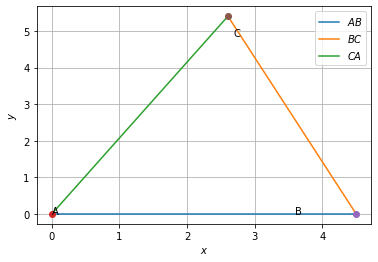
\includegraphics[width=\columnwidth]{solutions/triangle/10/download .png}
    \caption{ $\triangle ABC$}
    \label{tri/10/fig:triangle ABC}
\end{figure}
